\section{Alpha/Beta Pruning} 
\label{sec:Alpha/Beta Pruning}

\subsection{Introduction to Alpha/Beta Pruning}
\label{subsec:Introduction to Alpha/Beta Pruning}
Alpha/Beta pruning is the way by which the Minimax Algorithm is made more efficient.
This happens by stopping consideration of possible moves, that will never be better than previously considered moves.

\subsection{Explanation of Alpha/Beta Pruning}
\label{subsec:Explanation of Alpha/Beta Pruning}
Alpha Beta Pruning is an optimization method for the Minimax algorithm that eliminates branches or entire subtrees. 
It is so named because it introduces the two variables or values Alpha and Beta into the Minimax algorithm.
The variable Alpha is set to be the biggest value the Maximizer can guarantee at the current level being explored or above it.
The variable Beta is likewise set to be the smallest value the Minimizer can guarantee.

\begin{figure}
    \caption{An example of Alpha Beta Pruning} % Caption on top of both of the images.
    \label{fig:AlphaBetaPruningA}
    \centering % Centering requirement met
    \begin{subfigure}[b]{0.3\textwidth}
        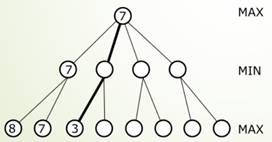
\includegraphics[width=\textwidth]{AlphaBetaPruning1.png}           
    \end{subfigure}
    \begin{subfigure}[b]{0.3\textwidth}
        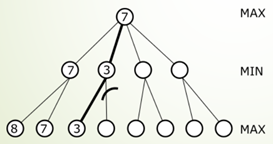
\includegraphics[width=\textwidth]{AlphaBetaPruning2.png}       
    \end{subfigure}
  \end{figure}

Figure \ref{fig:AlphaBetaPruningA} shows how first the leftmost branches are explored 
and the minimizer picks “7” which is stored in the variable Alpha. 
After that the second leftmost branch is explored and the Minimizer is presented with a choice that is smaller than 7.
Given that there is a choice smaller than Alpha present already, and it is the Minimizer’s turn to choose, 
meaning that it will undoubtedly have a chance to pick a value smaller than Alpha, 
it would not be worth it for the Maximizer to explore the rest of the branch and the branch is pruned as seen 
in figure \ref{fig:AlphaBetaPruningA}.

\begin{figure}
    \caption{An example of branches being pruned} % Caption on top of both of the images.
    \label{fig:AlphaBetaPruningB}
    \centering % Centering requirement met
    \begin{subfigure}[b]{0.3\textwidth}
        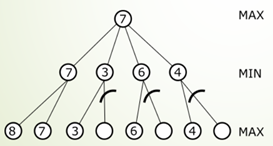
\includegraphics[width=\textwidth]{AlphaBetaPruning3.png}
    \end{subfigure}
    \begin{subfigure}[b]{0.3\textwidth}
        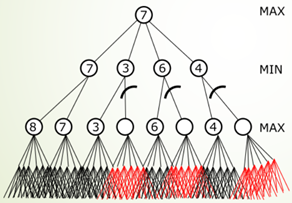
\includegraphics[width=\textwidth]{AlphaBetaPruning4.png}
    \end{subfigure}
  \end{figure}

  Alpha Beta Pruning can potentially prune a lot of branches and 
  thus make the examination of choices or moves through Minimax considerably faster 
  than if it simply went through every single branch.

\subsection{Implementation of Alpha/Beta Pruning}
\label{subsec:Implementation of Alpha/Beta Pruning}
% Show our new code!

\clearpage